%% -*- coding: utf-8 -*-
\documentclass[12pt,pagesize,paper=192mm:108mm,landscape]{scrbook} 
%1920x1080 1280x720
\areaset[current]{192mm}{108mm}
\usepackage{calc}
\usepackage[T2A]{fontenc}
\usepackage[utf8]{inputenc}
\usepackage[english,russian]{babel}
\usepackage{microtype}
\usepackage{misccorr}
\usepackage{cmap}
%\usepackage[unicode=true]{hyperref}
\usepackage{graphicx}
\usepackage{amssymb}
\usepackage{amsmath}
%\usepackage{srcltx}
\usepackage{textcomp}
\usepackage{xspace}
%научные символы и смайлики \smiley \frownie
\usepackage{wasysym}
\usepackage{ccicons}
%перенос формул в тексте
\newcommand*{\hm}[1]{#1\nobreak\discretionary{}%
  {\hbox{$\mathsurround=0pt #1$}}{}}

\begin{document}
\begin{titlepage}
  \vspace*{-0.5em}
  \begin{center}    
    % \hspace*{3em}
    % \begin{minipage}[t]{3em}
    %   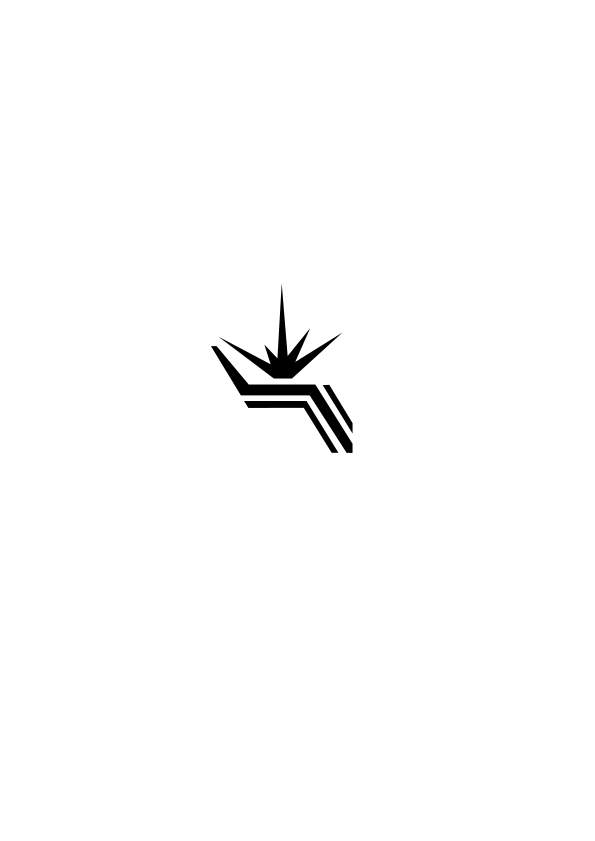
\includegraphics[width=\textwidth]{../BINP-logo}
    % \end{minipage}\hfill
    % \begin{minipage}{0.23\linewidth}
    % 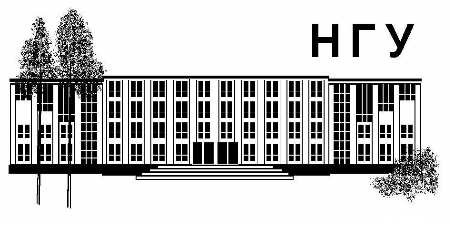
\includegraphics[width=\textwidth]{../NSU-logo}
    % \end{minipage}
    % \hfill
    % \hspace*{6em}

    % Кафедра теоретической физики физического факультета НГУ
    % \medskip

    % \Large
    % Профессор Грабовский А.\,В.
    % \smallskip

    % \huge
    % \textbf{Общая теория относительности}
    % \smallskip

    \vfill
    \Large
    Задание № 8
    \bigskip

    \normalsize
    \begin{minipage}{0.81\linewidth}
      \begin{enumerate}
      \item  Эффект Ленза"=Тирринга. Показать, что в поле Керра
        звезды с моментом $S_0$ на большом расстоянии от звезды $r$
        гироскоп с моментом $s$ прецессирует с~угловой скоростью
        $\Omega^k=G/(c^2r^3)\cdot(S_0^k-3(S_0r)r^k/r^2)$, то есть
        $ds^i/dt=\varepsilon_{ijk}\Omega^js^k$.
      \item Найти годовое изменение угла наклона момента импульса
        гироскопа, летающего вокруг Земли на полярной орбите с высотой
        $h=643$\,км, $T_{\text{обращения}}\hm{=}97{,}6$\,минут. Это параметры эксперимента
        Gravity Probe B. Сравнить полученные значения с
        экспериментальными данными GP-B: изменение угла за~счет
        геодезической прецессии "--- 6006{,}1'', за счет эффекта
        Ленза"--~Тирринга, то есть вращения Земли, "--- 39{,}2''. Объяснить,
        почему для этого эксперимента была выбрана полярная, а не
        экваториальная орбита.
      \item Получить изменение расстояния между близкими точками при
        прохождении гравитационной волны с помощью уравнения
        расхождения геодезических.
      \end{enumerate}
    \end{minipage}
    \vfill

    \normalsize \ccbysa\hspace{0.5em}  Новосибирск 2022
  \end{center}
\end{titlepage}
\end{document}
